\section{RESULTADOS E DISCUSSÕES}

%pré javascript

Nos primeiros dias da \emph{World Wide Web}, um navegador precisava apresentar apenas alguns tipos de dados aos usuários. Para não ser limitado por esses tipos de dados, os desenvolvedores trabalharam duro para estender os navegadores para que dados em outros formatos pudessem ser renderizados no computador cliente. Uma maneira de resolver o problema era permitir que o navegador, ao reconhecer um arquivo recebido de um tipo específico, iniciar um aplicativo separado na máquina cliente para renderizar o conteúdo. Desde que este aplicativo auxiliar tenha sido instalado no computador cliente, o navegador iniciará o programa e enviará o arquivo recebido para esse programa \cite{zammetti2007brief}.

A primeira solução para tornar a web mais dinâmica foi o \emph{“Common Gateway Interface”} (CGI), que permite a criação de programas que executem quando um usuário faz uma requisição. Porem, CGI não é a solução mais segura para criação de páginas web pois permite que seja executado um programa em seu sistema operacional e usuários maliciosos podem explorar isto com algum exploit\footnote{Uma sequência de comandos que tomam vantagem de um defeito, falha ou vulnerabilidade a fim de causar um comportamento acidental ou imprevisto.} e executar operações indesejadas \cite{Asleson2006}.

Ainda segundo \citeonline{Asleson2006}, em maio de 1995 John Gage e Andreessen anunciam o nascimento da linguagem de programação Java. O navegador Netscape era dominante na época e ofereceria suporte para esta nova linguagem. Dentro de alguns meses, milhares de pessoas já haviam baixado o Java em seus computadores, abrindo novos caminhos para páginas web dinâmicas.

Applets\footnote{Pequeno software que executa uma atividade específica dentro de outro programa maior.} permitem que pequenas aplicações Java possam ser incluídas nas páginas web e executadas através da \emph{Java Virtual Machine} (JVM). Applets são executadas no modelo de segurança de “caixa de areia” (\emph{sandbox}), não podem carregar bibliotecas nativas e são tipicamente impedidas de ler ou gravar no disco \cite{Asleson2006}.

% flash aqui

Ainda em maio de 1995, Brendan Eich, um funcionário da Netscape\footnote{Empresa de serviços de computadores nos EUA.} na época, desenvolveu uma linguagem de script em dez dias que se tornou conhecida como Mocha. Este nome original foi dado pelo fundador da Netscape. Pouco depois, o nome foi avaliado e renomeado como Livescript. Mais tarde naquele ano em dezembro, a Netscape recebeu uma licença de marca registrada da Sun\footnote{Fabricante de computadores, semicondutores e software com sede em Santa Clara, Califórnia, no Silicon Valley.}. Desta vez, o nome mudou para Javascript \cite{neer2013history}.

Javascript foi concebido para fins muito diferentes do Java, essencialmente para funcionar como uma linguagem de programação integrada em documentos HTML e não como uma linguagem para escrever applets que ocupam uma área retangular fixa na página \cite{goodman2007javascript}. O Javascript tinha um pequeno vocabulário e um modelo de programação mais facilmente digerível que o Java, com sua abordagem orientada a objetos. Nesse contexto \citeonline{crockford2008javascript} afirma que com Javascript é possível programar sem saber muito sobre a linguagem, ou mesmo saber muito sobre programação.

A primeira versão, o Javascript 1.0, estreou no navegador Netscape 2 em 1995. No momento do lançamento do Javascript 1.0, o Netscape dominava o mercado de navegadores. A Microsoft estava lutando para recuperar seu próprio navegador, Internet Explorer e seguiu rapidamente a liderança da Netscape ao lançar sua própria linguagem VBScript\footnote{Versão interpretada da linguagem Visual Basic para construção dinâmica de página HTML}, juntamente com uma versão do Javascript chamada JScript, com a entrega do Internet Explorer 3 \cite{keith2010dom}.

\begin{figure}[!htb]
	\centering
	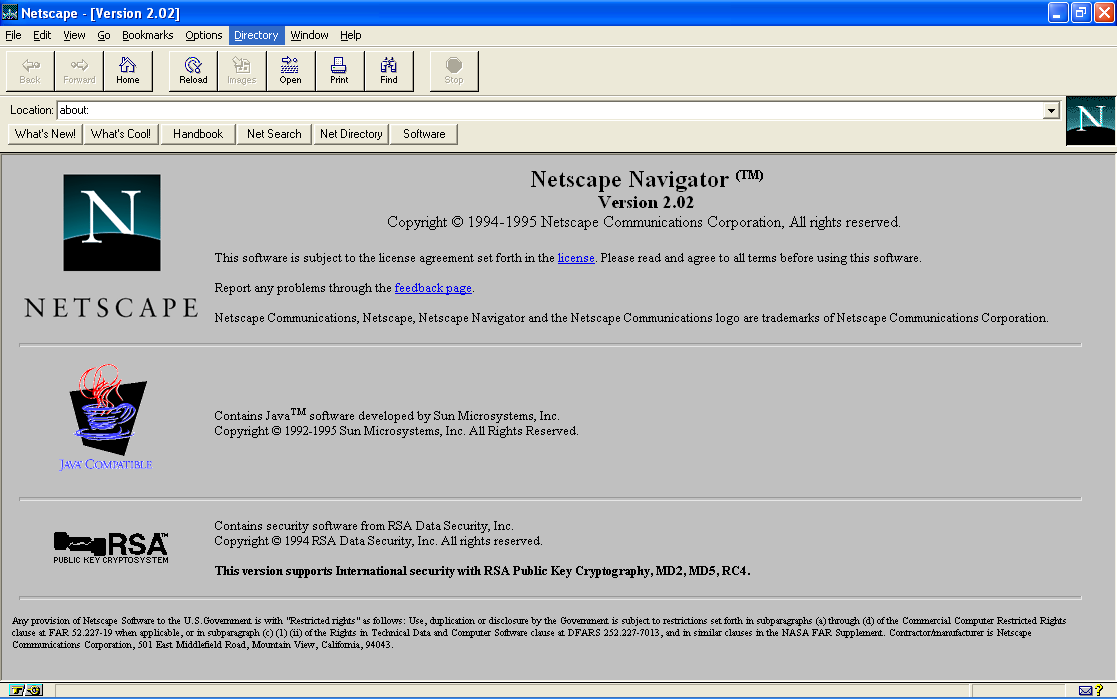
\includegraphics[width=350px]{Netscape_Navigator_2.png}
	\caption{Navegador Netscap 2}
	\label{fig:netscape}
\end{figure}

A Netscape enviou a linguagem para padronização para a Associação Europeia de Fabricante de Computadores (ECMA) e devido a problemas de marca registrada, a versão padronizada da linguagem estava presa com o nome estranho “ECMAScript”. Pelos mesmos motivos de marca registrada, a versão da Microsoft do idioma É formalmente conhecido como “JScript” \cite{flanagan2011javascript}.

O ECMAScript como foi padronizado não se destina a ser computacionalmente auto-suficiente, espera-se que o ambiente computacional de um programa ECMAScript forneça certos objetos específicos do ambiente; um navegador da Web fornece um ambiente de \emph{host} para computação do lado do cliente, incluindo, por exemplo, objetos que representam janelas, menus, pop-ups\footnote{Janela que abre no navegador da internet quando se acessa uma página na web ou algum link de redirecionamento.}, caixas de diálogo, áreas de texto, âncoras, quadros, histórico, cookies\footnote{Grupo de dados trocados entre o navegador e o servidor de páginas, colocado num arquivo de texto criado no computador do utilizador.} e entrada / saída; um servidor web fornece um ambiente de \emph{host} diferente para a computação do lado do servidor, incluindo objetos que representam requisições \cite{ecmascript2016}.

\subsection{Pré Ajax}

Em 1995, já era possível construir \emph{Single Page Applications} (SPAs) via frames/framesets\footnote{Divisões internas dentro de uma mesma janela do navegador, onde são carregados outros documentos HTML.} e url="javascript:...". Requisições assíncronas também eram possíveis utilizando Javascript e manipulando elementos HTML que realizavam requisições HTTP; praticamente qualquer tag que possa ser configurado para fazer referência a um URL pode ser empregado para tarefas de comunicação com base em Javascript \cite{powell2008ajax}.

Ainda segundo \citeonline{powell2008ajax}, utilizando-se de tags que referenciam URL é possível gerar uma requisição de via única ao servidor para indicar que algum evento aconteceu através de campos adicionados ao URL (\emph{Query Strings}). Para isso, utiliza-se de parâmetros passados via URL por uma tag\footnote{Estruturas de linguagem de marcação contendo instruções, tendo uma marca de início e outra de fim para que o navegador possa renderizar uma página.} \emph{<img>} por exemplo, cabe ao servidor tratar a requisição e retornar o dado esperado ou uma resposta vazia com status 204, informando ao cliente que a solicitação ocorreu sem erros mas que não há conteúdo na resposta.

Quanto ao uso da tag \emph{<img>} para comunicação bi-direcional \citeonline{powell2008ajax} completa:

\begin{citacao}
	Parece que o uso de uma imagem provavelmente não é a melhor maneira de transmitir informações bidirecionais. Considere que, se você pedir uma imagem, você estará recebendo uma imagem, provavelmente em formato GIF, JPEG ou PNG para exibição. Como exemplo, você pode solicitar ao usuário alguns dados e, em seguida, gerar uma imagem personalizada para eles. A transmissão dos dados fornecidos pelo usuário é através da sequência de consulta como anteriormente, mas desta vez o servidor responderá não com um código 204, mas com uma imagem real para usar. Você pode usar o DOM e inseri-lo na página.
\end{citacao}

Visto que um navegador permanecerá na mesma página quando receber uma resposta HTTP de status 204, ele pode ser usado para fingir ir a uma URL apenas para enviar alguns dados; isto é feito em Javascript com uma atribuição direta para \emph{window.location} enviando os dados pela URL, através das \emph{Query Strings}. Porem as \emph{Query Strings} são limitadas ao tamanho máximo da URL permitido pelo navegador.

Para envio de uma grande quantidade de dados o desenvolvedor precisaria realizar uma requisição HTTP POST com uma técnica de iframes\footnote{Elemento HTML que permite carregar as informações de um documento HTML separado em um documento HTML existente.} escondidos. Está técnica consiste da criação de campos de formulário a serem enviados com o formulário inserido no iframe. Uma vez que o formulário é preenchido com os dados desejados, é desencadeado o envio do formulário via Javascript.

A utilização de iframe é flexível no que pode receber em comparação com alguns dos outros métodos, permitindo a comunicação bi-direcional através de respostas em XHTML\footnote{Linguagem Extensível para Marcação de Hipertexto.}, XML\footnote{Linguagem de marcação para a criação de documentos com dados organizados hierarquicamente.}, JSON\footnote{Notação de Objetos JavaScript, é uma formatação leve de troca de dados.} ou outro formato de codificação à serem tratado com Javascript no navegador \cite{powell2008ajax}.

\subsection{Ajax}

O termo Ajax é um acrônimo para Javascript assíncrono e XML que segundo \citeonline{Garrett2005}, descreve uma maneira de realizar uma comunicação HTTP a partir de uma aplicação Javascript em páginas web.

Ajax é uma mistura do antigo com o novo, porque as tecnologias já existentes são combinadas em técnicas que pouco se considerava anteriormente, trazendo uma nova geração de aplicações é idéias \cite{gross2006introduction}.

Nesse contexto, \citeonline{Asleson2006} afirmam:
\begin{citacao}
	Honestamente, o Ajax não é nada novo. Na verdade, a tecnologia “mais nova” relacionada ao termo - o objeto XMLHttpRequest (XHR) - tem ocorrido desde o Internet Explorer 5 (lançado na primavera de 1999) como um controle ActiveX\footnote{Framework criado pela Microsoft que adapta as antigas versões das plataformas COM - Component Object Model e OLE - Object Linking and Embedding para conteúdo disponível online, especialmente aplicações web e cliente/servidor.}. No entanto, o que é novo é o nível de suporte do navegador. Originalmente, o objeto XHR era suportado apenas no Internet Explorer (limitando assim seu uso), mas, com o Mozilla 1.0 e Safari 1.2, o suporte é generalizado.
\end{citacao}

Criado pela Microsoft no fim da decada de 90, XMLHttpRequest é a interface através da qual o navegador pode fazer requisições HTTP com Javascript. Quando a interface XMLHttpRequest foi adicionada ao Internet Explorer, ele permitiu que os desenvolvedores fizessem coisas com o Javascript que antes era muito difícil \cite{haverbeke2014eloquent}.

Segundo \citeonline{grigorik2013high}, o XHR não apenas habilitou a comunicação assíncrona no navegador, mas também tornou mais simples esta, pois o XHR é uma API de aplicativos fornecida pelo navegador, o que significa que o navegador cuida automaticamente de todos os gerenciamentos de conexão de baixo nível.

Ainda segundo \citeonline{grigorik2013high}, o XHR tornou-se um padrão de fato em todos os principais navegadores porem o documento de especificação oficial só foi publicado em 2006 pelo \emph{World Wide Web Consortium} (W3C)\footnote{Principal organização de padronização da World Wide Web.}, bem depois de ter sido amplamente utilizado.

De fato, o envio de dados assíncronos ao servidor e a recepção de dados adicionais são o objetivo final do Ajax. Todos os processos do Ajax começam com uma conexão com o servidor. As conexões ao servidor geralmente são organizadas através do objeto XMLHttpRequest \cite{resig2007pro}.

\begin{figure}[!htb]
	\centering
	\subfloat[Modelo clássico de aplicação WEB  (síncrono)]{
		\raisebox{0.15\height}{
			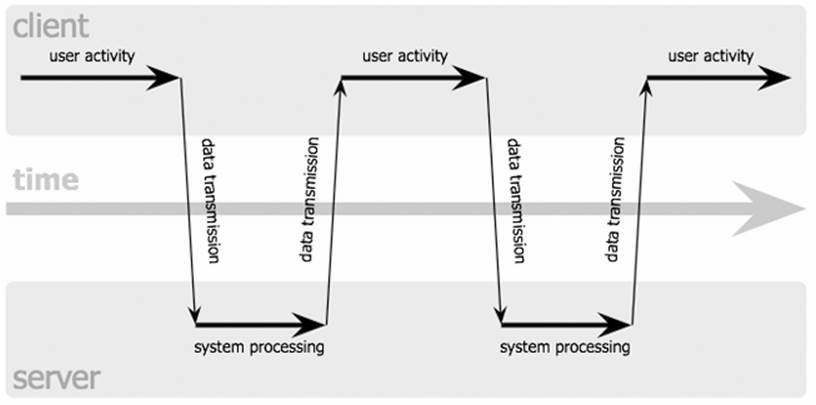
\includegraphics[width=210px]{default-pattern.jpg}
		}
		\label{defaultPattern}
	}
	\hfill
	\subfloat[Modelo de aplicação WEB Ajax (assíncrono)]{
		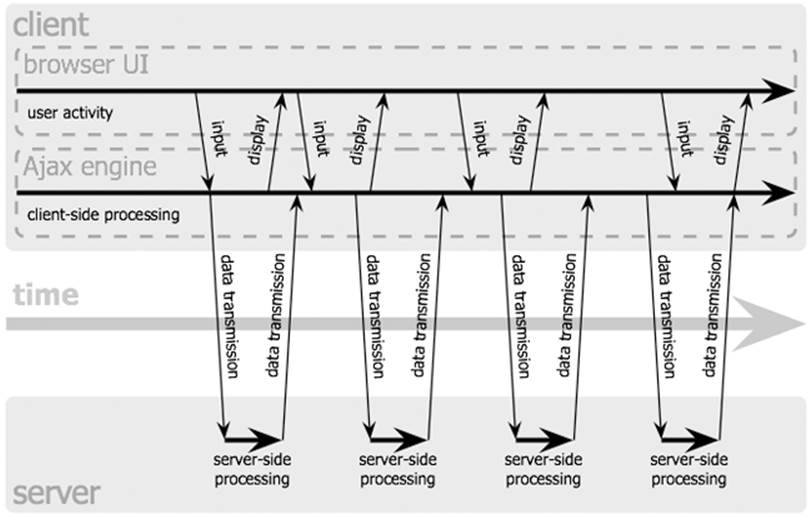
\includegraphics[width=210px]{ajax-pattern.png}
		\label{ajaxPattern}
	}
	\caption{Comparação entre o modelo clássico e o modelo Ajax}
	\label{defaultVsAjax}
\end{figure}

\begin{citacao}
	As versões iniciais do XHR proporcionaram recursos limitados: transferências de dados baseadas em texto, suporte restrito para o processamento de uploads e incapacidade de lidar com solicitações entre domínios\footnote{Nome que serve para localizar e identificar conjuntos de computadores na internet}. Para resolver essas falhas, o rascunho “XMLHttpRequest Level 2” foi publicado em 2008, que adicionou uma série de novos recursos \cite[P.~262-263]{grigorik2013high}.
\end{citacao}

Todos os novos recursos e recursos XHR2 são oferecidos através da mesma API XMLHttpRequest. Hoje, há apenas uma especificação XHR unificada, pois em 2011 a especificação “XMLHttpRequest Level 2” foi mesclada com a especificação original \cite{grigorik2013high}.

Uma lista de compatibilidade com os principais navegadores do mercado, pode ser conferida na Figura \ref{fig:xhr2}.

\begin{figure}[!htb]
	\centering
	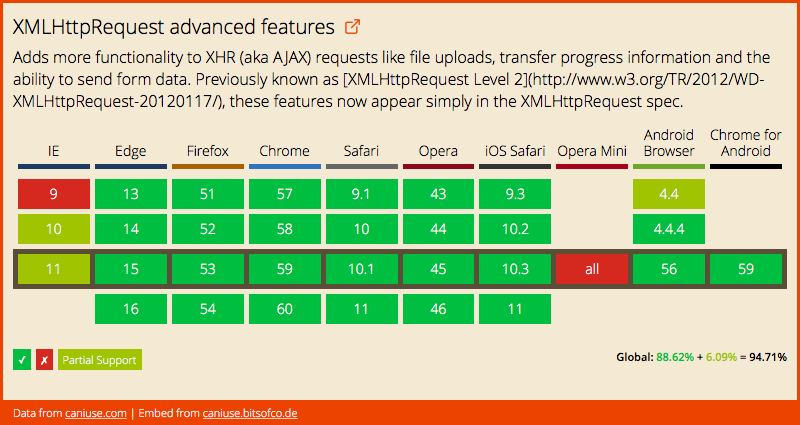
\includegraphics[width=400px]{XMLHttpRequest.png}
	\caption{Navegadores compatíveis com XHR2}
	\label{fig:xhr2}
\end{figure}

\subsection{HTTP Polling}

Segundo \citeonline[P.~273]{grigorik2013high}, “o HTTP não fornece nenhuma maneira para o servidor iniciar uma nova conexão com o cliente”. Para isso, o cliente deve pesquisar por atualizações no servidor.

Para uma atualização constante de informações entre o cliente e servidor, XHR nos fornece uma maneira simples. O cliente faz uma solicitação regular ao servidor solicitando atualizações e o servidor responde, podendo a resposta não conter dado. Esta técnica é conhecida por \emph{Polling HTTP} (ou \emph{Ajax Polling}). Tende a ser um desperdício de recursos de rede e de servidor, porem é fácil de implementar \cite{mccarthy2009comet}.

No entanto, de acordo com \citeonline{Pimentel2012}, \emph{Polling HTTP} é considerada uma boa solução para a entrega de informações em tempo real se o intervalo de entrega da mensagem for conhecido e  a taxa de transmissão de dados for constante. Porem, a cada consulta HTTP, repete-se informações de cabeçalho aumentando assim a latência.

Para reduzir a latência sem aumentar a carga do servidor, a solução é criar dois fluxos de comunicação entre o cliente e o servidor em uma técnica conhecida por \emph{Long Polling HTTP}. O primeiro fluxo é usado para receber mensagens e o segundo fluxo é usado para enviar mensagens. Para receber mensagens, o cliente pesquisa o servidor com um pedido de mensagens; se não houver mensagens, o servidor não responde com uma resposta imediatamente. O servidor coloca o pedido de pesquisa em espera por um período de tempo específico ou até que uma mensagem seja gerada pelo servidor  (Figura \ref{fig:longPolling}). A redução da latência é significativa, ao converter o tempo inoperante em uma espera criada pelo servidor, enquanto o cliente aguarda o potencial de uma mensagem que está sendo gerada \cite{gross2006introduction}.

\begin{figure}[!htb]
	\centering
	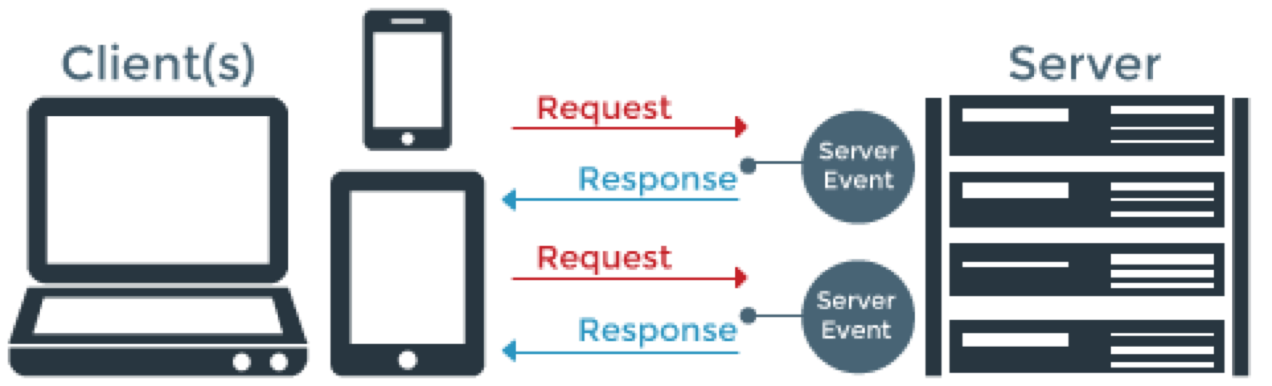
\includegraphics[width=400px]{Long-Polling.png}
	\caption{Long Polling HTTP}
	\label{fig:longPolling}
\end{figure}

Ainda segundo \citeonline{gross2006introduction}, o principal problema desta abordagem é que milhares de threads\footnote{Pequeno programa que trabalha como um subsistema, sendo uma forma de um processo se auto dividir em duas ou mais tarefas.} podem estar aguardando mensagens que possam ou não ser geradas, consumindo uma grande quantidade de Memória RAM\footnote{Tecnologia que permite o acesso aos arquivos armazenados no computador, responsável pela leitura dos conteúdos quando requeridos.}.

Nesta técnica, a conexão entre o cliente e servidor fica ociosa até expirar ou até que o servidor tenha dados para enviar. Cabe ao cliente a responsabilidade pela reconexão para aguardar a próxima atualização. Esta técnica é mais eficiente que \emph{Ajax Polling}, quando os dados são enviados com pouca frequência \cite{gutwin2011real}.

\subsection{HTTP Streaming}

Esta técnica se aproveita de um tipo de conteúdo HTTP chamado “\emph{multipart}” que permite que um servidor web envie conteúdo para um navegador em várias peças (\emph{chunked encoding}), projetada para o carregamento incremental de documentos muito grandes \cite{gutwin2011}.

A implementação mais simples desta técnica é conhecida por \emph{ForeverFrame}, onde tem-se um iframe dentro de uma página HTML recebendo atualizações constantes através do recebimento de partes de dados contendo uma mensagem completa em cada parte. Inicialmente esta técnica foi bastante condenada no Internet Explorer, pois este trata cada fragmento recebido como uma carga de página, disparando então, som de clique, do carregamento de página. A solução veio com a utilização do objeto \emph{htmlfile}\footnote{Interface para obter informações, examinar e modificar documentos HTML.} do ActiveX, tornando a técnica bastante popular \cite{souders2009even}.

Esta técnica também pode ser explorada em uma requisição XHR (\emph{XHR Streaming}), permitindo que um servidor web envie conteúdo para um navegador em várias partes. Essencialmente, o navegador é enganado para manter a conexão do soquete aberta, com o servidor enviando cada atualização como parte de um todo. O uso de uma única conexão de soquete também reduz o número de cabeçalhos HTTP que precisam ser enviados para pedidos e respostas, reduzindo assim, a latência.

\subsection{Server-Sent Event (SSE)}

Proposto desde 2009, define uma API para abrir uma conexão HTTP para receber notificações \emph{push}\footnote{Sistema de distribuição de conteúdo da Internet em que a informação sai de um servidor para um cliente, com base em uma série de parâmetros estabelecidos pelo cliente.} de um servidor na forma de eventos DOM, permitindo que os servidores enviem dados para páginas da Web por meio de HTTP ou usando protocolos dedicados de envio \cite{hicksonserver2015}.

Normatizado pelo W3C em fevereiro de 2015, apresenta a interface \emph{EventSource}; é projetada de modo que possa ser estendida para funcionar com outros esquemas de notificação \emph{push}, como \emph{Push SMS}\footnote{Serviço utilizado para o envio de mensagens de texto curtos, através de telefones celulares.} \cite{hicksonserver2015}.

\begin{citacao}
	Sob o capô, SSE oferece uma implementação eficiente e cruzada do \emph{XHR Streaming}; A entrega real das mensagens é feita através de uma única conexão HTTP de longa duração. No entanto, ao contrário de lidar com transmissão de XHR por conta própria, o navegador lida com todo o gerenciamento de conexão e análise de mensagens, permitindo que nossos aplicativos se concentrem na lógica de negócios! Em suma, a SSE torna o trabalho com dados em tempo real simples e eficiente \cite[P.~279]{grigorik2013high}.
\end{citacao}

Suportado nativamente pela maioria dos navegadores modernos (Figura \ref{fig:sse}); foi uma adição antecipada à especificação HTML5. No entanto, a interface \emph{EventSource} é simples, de modo que pode ser emulada através de uma biblioteca de Javascript opcional (\emph{Polyfill}\footnote{Biblioteca Javascript que implementa o padrão HTML5, quer seja um padrão estabelecido para todos os navegadores ou não.}) para navegadores que não o suportam nativamente \cite{grigorik2013high}.

\begin{figure}[!htb]
	\centering
	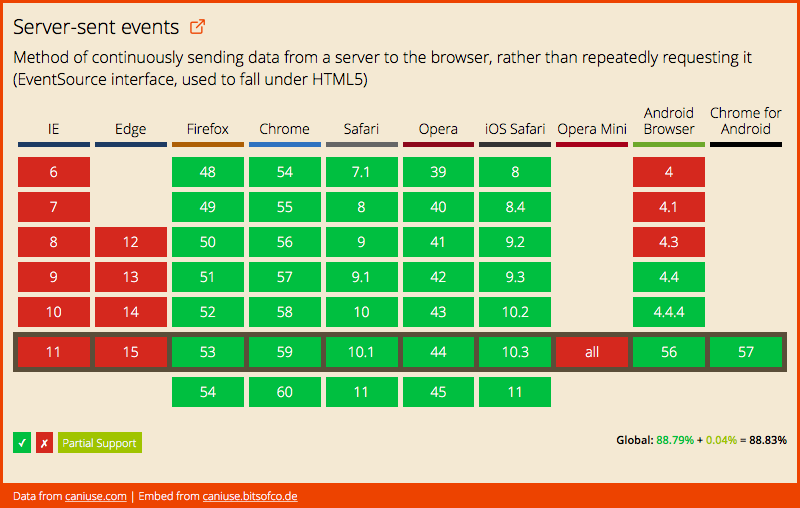
\includegraphics[width=400px]{Can_I_Use-SSE.png}
	\caption{Navegadores compatíveis com Server-Sent Event}
	\label{fig:sse}
\end{figure}

% TODO: Completar o texto
------------------------------------------------------------------------------------
------------------------------- PAREI AQUI ----------------------------------------
------------------------------------------------------------------------------------

\subsection{Web Sockets}

% TODO: Esse kra vai ficar por ultimo